\documentclass{article}

\usepackage{graphicx}
\usepackage{tikz}
\usepackage{tikzsymbols}
\usetikzlibrary{calc,patterns,shapes.geometric}
\pagestyle{empty}
\usepackage[margin=0pt]{geometry}
\geometry{papersize={14in,12in}}

\def\centerarc[#1](#2)(#3:#4:#5){\draw[#1] ($(#2)+({#5*cos(#3)},{#5*sin(#3)})$) arc (#3:#4:#5);}

\begin{document}
	\begin{figure}
		\centering
		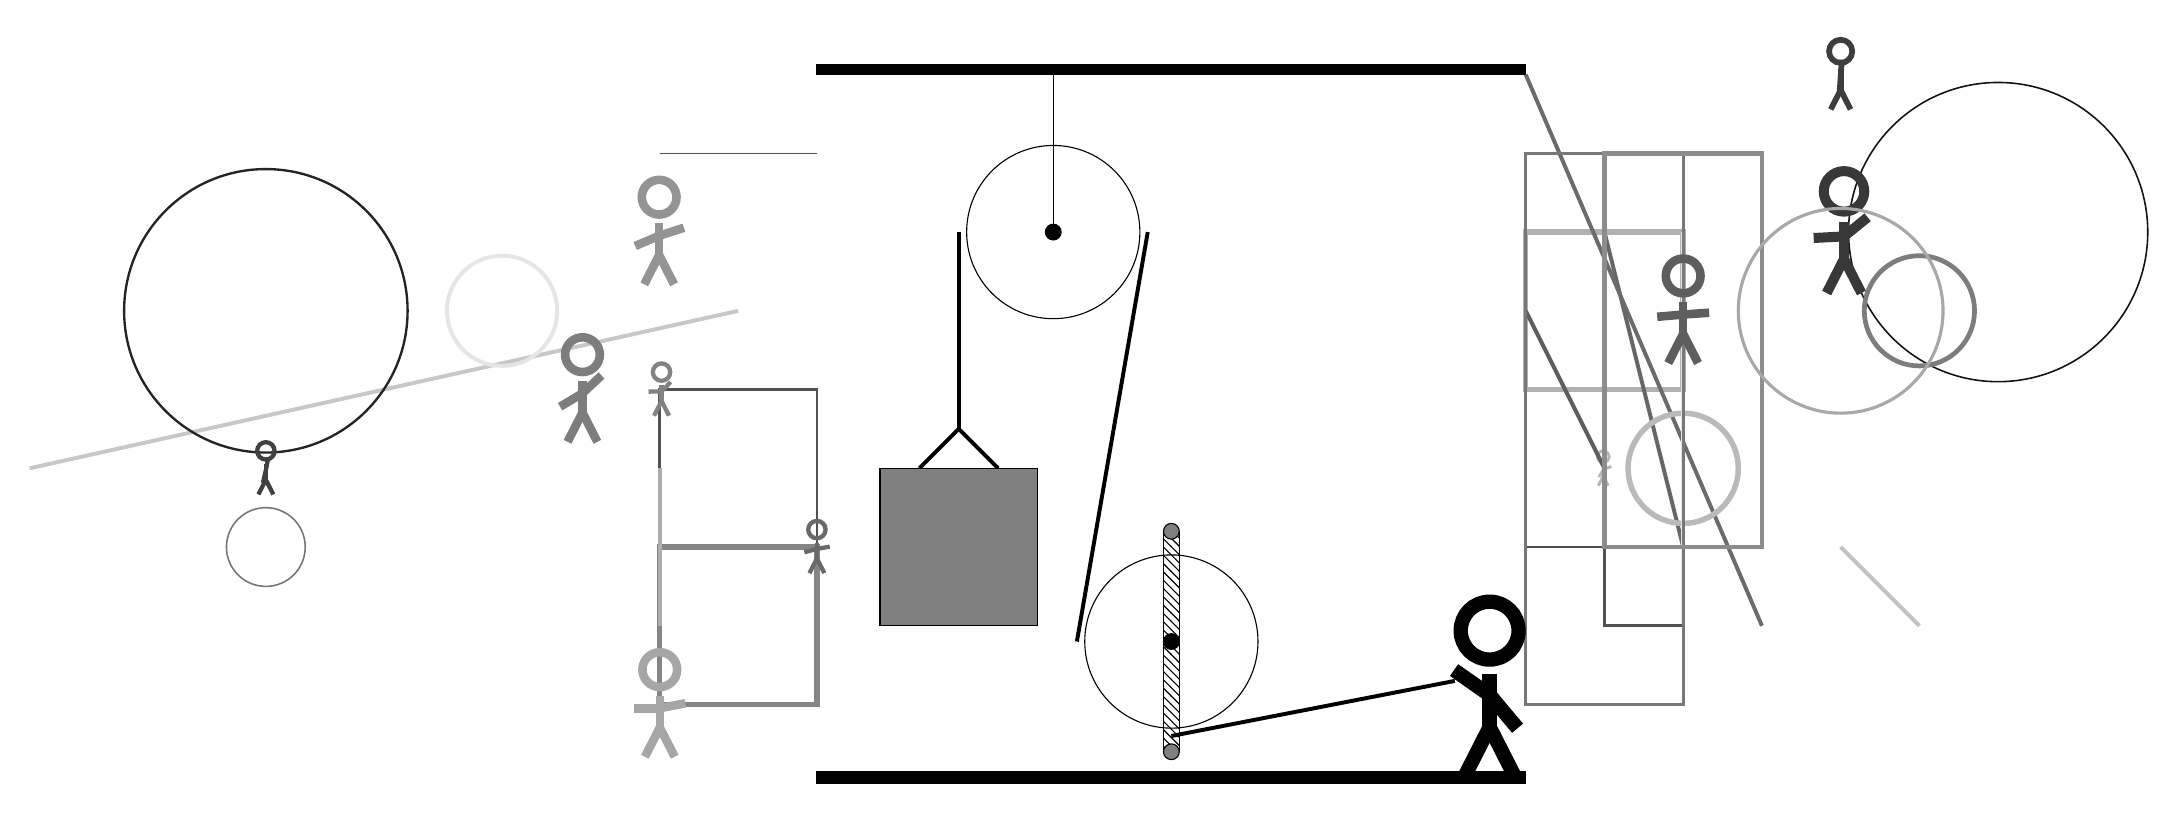
\begin{tikzpicture}
			%%%%% START %%%%%
			
			\draw[fill=black] (-2, 9) rectangle (7, 9.125);
			
			\draw[line width=0.5mm, color=black!22](-3, 6) -- (-12, 4);
			
			\draw[line width=0.3mm, color=black!68] (-2, 1) rectangle (-4, 5);
			\draw [line width=0.3mm, color=black!86](-9, 6) circle (1.8);
			\draw[line width=0.2mm, color=black!70] (7, 3) rectangle (8, 3);
			
			\draw [line width=0.2mm, color=black!93](13, 7) circle (1.9);
			\draw[line width=0.7mm, color=black!31] (9, 7) rectangle (7, 5);
			
			\draw[line width=0.2mm, color=black!68] (-4, 8) rectangle (-2, 8);
			
			\node[line width=0.7mm, color=black!42] at (-4, 7) {\Strichmaxerl[6][23][18]};
			\draw[line width=0.5mm, color=black!60](9, 3) -- (8, 7);
			\draw[line width=0.5mm, color=black!58](10, 2) -- (7, 9);
			\node[line width=0.2mm, color=black!29] at (8, 4) {\Strichmaxerl[2][60][21]};
			
			\draw[line width=0.7mm, color=black!48] (-4, 1) rectangle (-2, 3);
			\draw[line width=0.5mm, color=black!24](12, 2) -- (11, 3);
			\draw [line width=0.7mm, color=black!27](9, 4) circle (0.7);
			\draw [line width=0.4mm, color=black!96](10, 2) circle (0.0);
			\node[line width=0.2mm, color=black!35] at (-4, 1) {\Strichmaxerl[6][0][11]};
			
			\draw [line width=0.6mm, color=black!51](12, 6) circle (0.7);
			\draw[line width=0.5mm, color=black!63](8, 4) -- (7, 6);
			\draw[line width=0.5mm, color=black!32](-4, 4) -- (-4, 2);
			
			\node[line width=0.6mm, color=black!75] at (-9, 4) {\Strichmaxerl[3][77][79]};
			\draw[line width=0.5mm, color=black!10](9, 2) -- (9, 7);
			
			\draw[line width=0.4mm, color=black!68] (8, 2) rectangle (9, 3);
			\node[line width=0.3mm, color=black!78] at (11, 7) {\Strichmaxerl[7][3][39]};
			\draw[line width=0.4mm, color=black!53] (9, 8) rectangle (7, 1);
			\draw[line width=0.6mm, color=black!45] (8, 8) rectangle (10, 3);
			
			\node[line width=0.4mm, color=black!59] at (-2, 3) {\Strichmaxerl[3][15][10]};
			
			\node[line width=0.4mm, color=black!51] at (-5, 5) {\Strichmaxerl[6][31][43]};
			\draw [line width=0.2mm, color=black!54](-9, 3) circle (0.5);
			\draw [line width=0.4mm, color=black!34](11, 6) circle (1.3);
			\node[line width=0.6mm, color=black!49] at (-4, 5) {\Strichmaxerl[3][1][46]};
			\draw [line width=0.5mm, color=black!10](-6, 6) circle (0.7);
			
			\node[line width=0.6mm, color=black!63] at (9, 6) {\Strichmaxerl[6][5][4]};
			\node[line width=0.3mm, color=black!76] at (11, 9) {\Strichmaxerl[4][86][86]};
			
			\draw (1, 7) circle (1.1);
			\draw[fill=black] (1, 7) circle (0.1);
			\draw (1, 9) -- (1, 7);
			
			\draw[fill=white](2.5, 1.8) circle (1.1);
			\draw[fill=black] (2.5, 1.8) circle (0.1);
			\draw[pattern=north west lines, pattern color=black] (2.4, 3.2) rectangle (2.6, 0.4);
			\draw[fill=black!50] (2.5, 3.2) circle (0.1);
			\draw[fill=black!50] (2.5, 0.4) circle (0.1);
			
			\draw[line width=0.5mm] (-0.7, 4.0) -- (-0.2, 4.5) -- (0.3, 4.0);
			\draw[fill=black!50] (-1.2, 4.0) rectangle (0.8, 2.0);
			
			\draw[line width=0.5mm] (-0.2, 7) -- (-0.2, 4.5);
			\centerarc[line width=0.5mm](1, 7)(0:180:1.2000000000000002);
			\draw[line width=0.5mm](2.2, 7) -- (1.3, 1.8);
			\centerarc[line width=0.5mm](2.5, 1.8)(180:270:1.2000000000000002);
			\draw[line width=0.5mm](2.5, 0.6) -- (6.1, 1.3);
			
			\node at (6.5, 1.2) {\Strichmaxerl[10][-35][-50]};
			
			\draw[fill=black] (-2, 0) rectangle (7, 0.15);
			
			%%%%% END %%%%%
		\end{tikzpicture}
	\end{figure}	
\end{document}